\subsection{The Code}
My project is consisted of the following components:

\begin{table}[H]
    \centering
    \begin{tabular}{ll}
        \midrule
        \textbf{doc} & Documentation, source and pdf  \\
        \textbf{out} & Saved Checkpoint - model \& state dict. \\
        \textbf{samples} & Test images for Demo \\
        \textbf{src} & Project's sources \\
        \textbf{support} & Dockerfile to reproduce the required env. \\
        \bottomrule
    \end{tabular}
    \caption{}
    \label{tab:}
\end{table}


\begin{table}[H]
    \centering
    \begin{tabular}{ll}
        \midrule
        \textbf{Camera.py} & Capture frames from Camera or a Video  \\
        \textbf{FaceMaskClassificationUtils.py} & Shared Helper and constants  \\
        \textbf{FaceMaskDetection.py} & FaceMask classifier model   \\
        \textbf{FinalProject.py} & train and classify without a GUI \\
        \textbf{Gui.py} & A useful GUI assisting upload and classify images \\
        \textbf{HumanDetection.py} & Human Detection Model \\
        \textbf{ObjectCrop.py} & External Lib For Objects Detection \\
        \bottomrule
    \end{tabular}
    \caption{}
    \label{tab:2}
\end{table}

\subsection{How To Run The Project}
\begin{itemize}
\item Train the model and test it, export a checkpoint file for the model and weights
\begin{verbatim}
$$ python src/FinalProject.py --help
optional arguments:
  -h, --help            show this help message and exit
  -H HUMAN_MODEL_PATH, --human_model_path HUMAN_MODEL_PATH
                        Human Model Path
  -a HUMAN_DATA_PATH, --human_data_path HUMAN_DATA_PATH
                        Human Data Path
  -M MASK_MODEL_PATH, --mask_model_path MASK_MODEL_PATH
                        Face Mask Model path
  -b MASK_DATA_PATH, --mask_data_path MASK_DATA_PATH
                        Face Mask Data path
  -F IMAGE_PATH, --image_path IMAGE_PATH
                        image to classify
  --train
\end{verbatim}

\item{Run GUI to classify images selected by the user:}
\begin{verbatim}
$$ python src/Gui.py --help
optional arguments:
  -h, --help            show this help message and exit
  -H HUMAN_MODEL_PATH, --human_model_path HUMAN_MODEL_PATH
                        Human Model Path
  -M MASK_MODEL_PATH, --mask_model_path MASK_MODEL_PATH
                        Face Mask Model path
\end{verbatim}
    \item{Run Video/Camera capture and classify frames}
    \begin{verbatim}
$$ python src/Camera.py
usage: Camera.py [-h] -H HUMAN_MODEL_PATH -M MASK_MODEL_PATH -F VIDEO_PATH
                 [--skip_capturing]

    \end{verbatim}
\end{itemize}

Prerequisites:
\begin{itemize}
    \item Pre trained model checkpoint (Model \& weights)
    \item Project's Python source code
\end{itemize}

\subsection{Demo Agena}
\subsubsection{Textual}
\begin{verbatim}
$ cd ~/Project/ && time python src/FinalProject.py \
                        -H out_models/CombinedModel2.pth \
                        -M out_models/MaskModel2.pth \
                        -a data/human/ -b data/face-mask/ \
                        -N out_models/NaturalNodel2.pth \
                        -c data/natural_images \
                        -F samples/nre/Partial.jpg
\end{verbatim}
\begin{figure}[H]
    \centering
    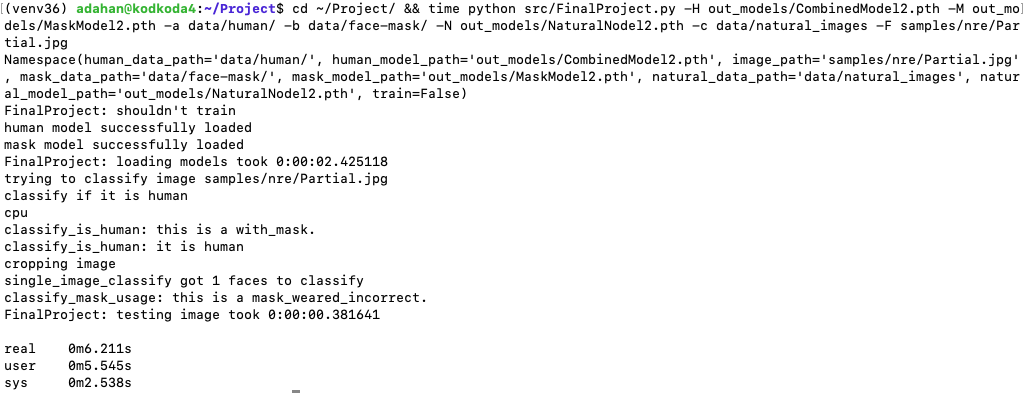
\includegraphics[width=1\textwidth]{images/Demo/Textual.png}
    \caption{Cropping Sample}
    \label{fig:Textual}
\end{figure}
\subsubsection{Gui}
\begin{verbatim}
$ cd ~/Project/ && python src/Gui.py \
                   -H out_models/CombinedModel2.pth \
                   -M out_models/MaskModel2.pth
\end{verbatim}
I'll attach here samples of my self Gui tests:
\begin{figure}[H]
    \centering
    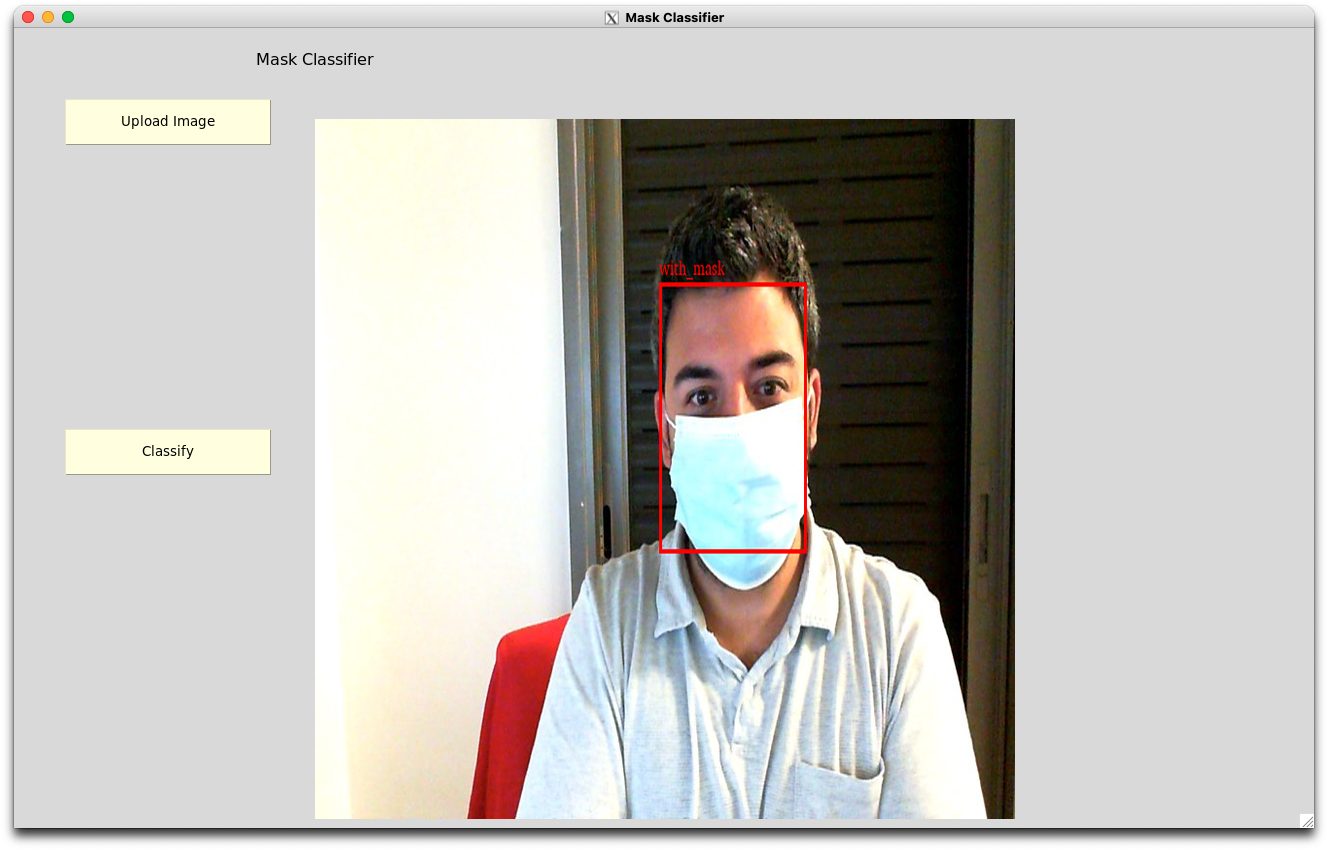
\includegraphics[width=0.5\textwidth]{images/Demo/Masked.png}
    \caption{Amir is with his mask ON}
    \label{fig:MaskedAmir}
\end{figure}

\begin{figure}[H]
    \centering
    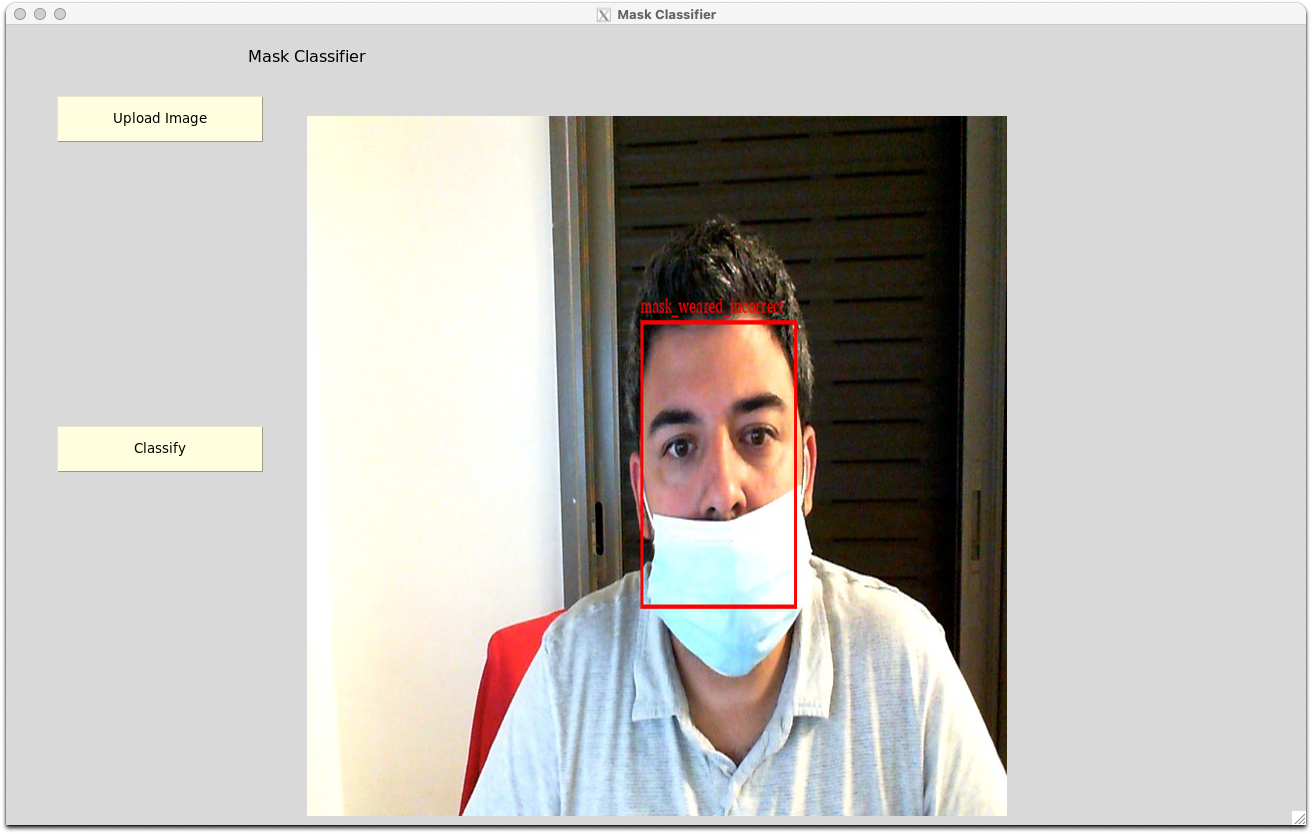
\includegraphics[width=0.5\textwidth]{images/Demo/Partial.png}
    \caption{Amir is with his mask Partially ON}
    \label{fig:PartialMaskedAmir}
\end{figure}
\begin{figure}[H]
    \centering
    \includegraphics[width=0.5\textwidth]{images/Demo/Unmasked.png}
    \caption{Amir is with his mask OFF}
    \label{fig:UnMaskedAmir}
\end{figure}
\begin{figure}[H]
    \centering
    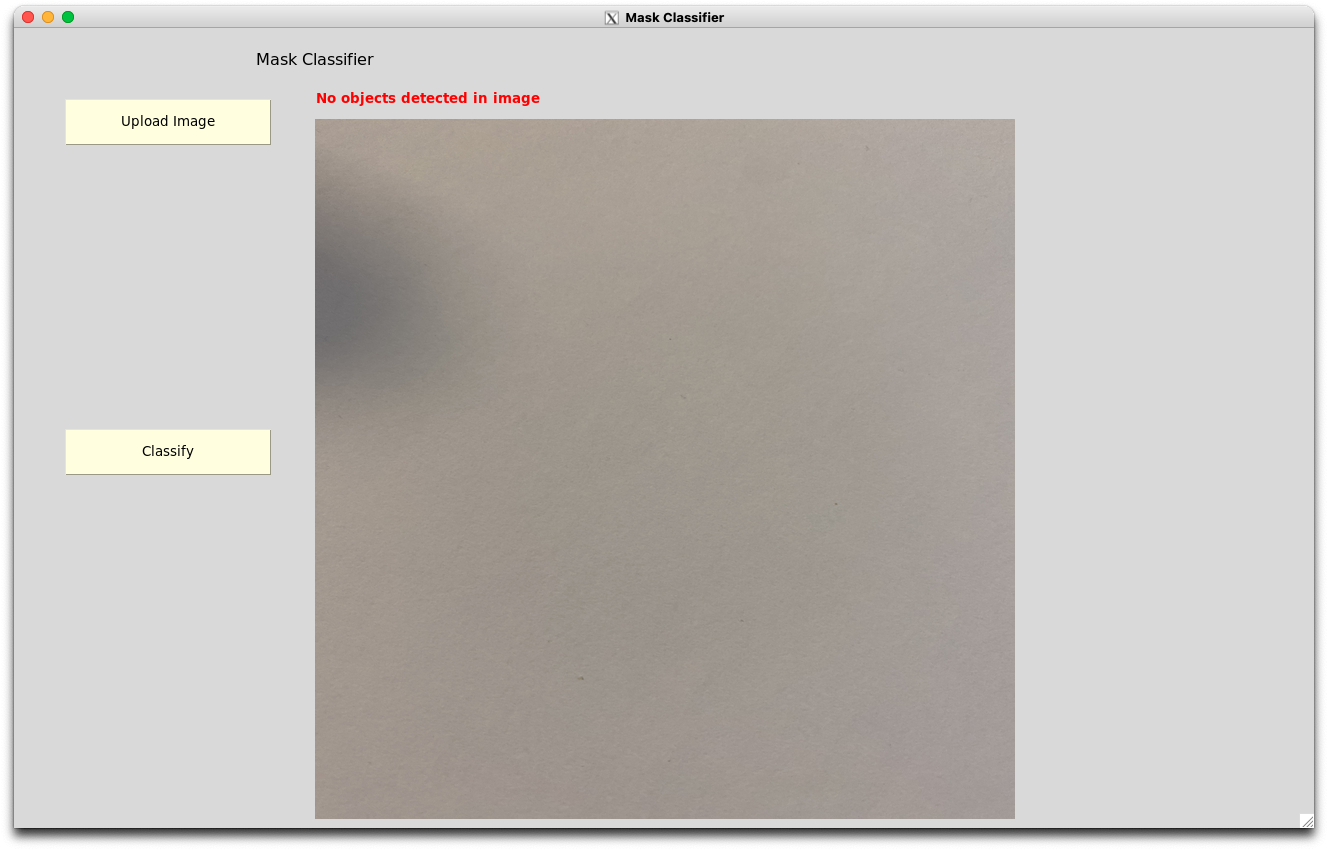
\includegraphics[width=0.5\textwidth]{images/Demo/wall.png}
    \caption{A blank wall}
    \label{fig:Wall}
\end{figure}
\begin{figure}[H]
    \centering
    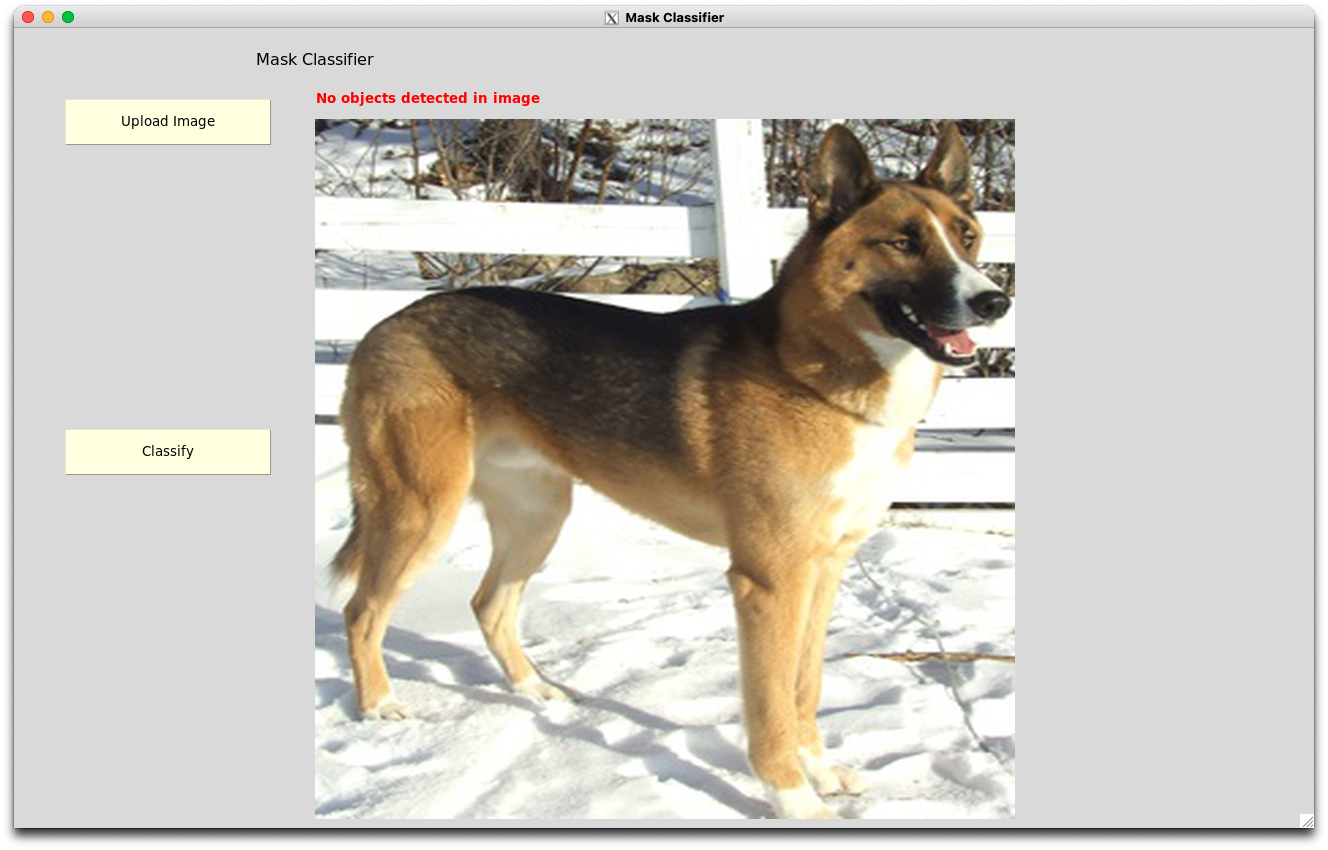
\includegraphics[width=0.5\textwidth]{images/Demo/dog.png}
    \caption{A Dog}
    \label{fig:Dog}
\end{figure}
\subsubsection{Video}
\begin{verbatim}
$ cd ~/Project/ && python src/Camera.py \
                   -H out_models/CombinedModel2.pth \
                   -M out_models/MaskModel2.pth \
                   -F samples/nre/Movie.mov --skip
\end{verbatim}
